\chapter{Contesto di Riferimento e Stato dell'Arte}
\label{ch:bck_rltd_wrks}

\section{Telecomunicazioni terrestri e satellitari}
\label{sec:telecomunicazioni}

L'evoluzione delle infrastrutture di rete ha trasformato i sistemi di telecomunicazione nei pilastri portanti della società moderna, la cui resilienza costituisce un prerequisito fondamentale per la sicurezza delle infrastrutture critiche e la continuità dei servizi essenziali \cite{tanenbaum2020}. 
Con il passaggio a un paradigma trasmissivo interamente digitale, la convergenza di vettori elettrici, ottici ed elettromagnetici su tratte geografiche complesse ha determinato un ampliamento esponenziale della superficie d'attacco\footnote{Con superficie d'attacco si intende l'insieme complessivo dei punti di accesso, vulnerabilità software, interfacce di rete e nodi fisici attraverso cui un agente malevolo può tentare di accedere o alterare un sistema di telecomunicazione.}. 
La compromissione o la degradazione intenzionale di un canale di comunicazione non comporta soltanto una temporanea perdita di connettività, ma può innescare disservizi sistemici a cascata, compromettendo l'integrità dei dati e paralizzando processi decisionali in tempo reale \cite{stallings2020}. 
In un contesto caratterizzato da minacce informatiche ad alta persistenza, la sicurezza dei vettori di trasmissione deve quindi configurarsi come un requisito di progettazione nativo (\textit{security-by-design}), orientato a garantire la riservatezza, l'autenticità e la disponibilità dei flussi informativi. 
Tale imperativo difensivo richiede una disamina puntuale dei vincoli strutturali e dei profili di rischio propri dei diversi domini trasmissivi, a partire dall'analisi delle reti di superficie.

\paragraph{Telecomunicazioni terrestri}

In questo quadro, la strutturazione delle infrastrutture di comunicazione terrestri evidenzia un profondo compromesso tra efficienza prestazionale e complessità delle contromisure di sicurezza. 
Da un lato, la combinazione di mezzi guidati ad altissimo throughput, come le fibre ottiche, e di vettori radio a frequenze elevate garantisce latenze di propagazione ridottissime, rendendo tali reti il supporto d'elezione per applicazioni a bassa latenza e in tempo reale \cite{tanenbaum2020}. 
Dall'altro, la natura distribuita e fisicamente accessibile dei nodi di rete espone l'infrastruttura a un ampio spettro di minacce: la presenza di tratte cablate e apparati di instradamento intermedi moltiplica le superfici d'attacco, agevolando sia intercettazioni fisiche sia attacchi logici di tipo \textit{Man-in-the-Middle} e \textit{Denial of Service} (DoS) \cite{stallings2020}. 
Sebbene i protocolli crittografici di rete e trasporto (quali IPsec e TLS\footnote{IPsec (\textit{Internet Protocol Security}) opera a livello di rete (Livello 3 del modello ISO/OSI) cifrando direttamente i pacchetti IP, mentre TLS (\textit{Transport Layer Security}) agisce a livello di trasporto/sessione (Livelli 4--5 ISO/OSI) per proteggere il canale di comunicazione sopra TCP.}) garantiscano la riservatezza e l'integrità dei dati contro l'ascolto passivo, essi si dimostrano intrinsecamente insufficienti a proteggere le infrastrutture complesse. 
Da un lato, non ostacolano l'analisi del traffico e dei metadati\footnote{L'analisi del traffico (\textit{traffic analysis}) consiste nell'estrazione di informazioni sensibili tramite l'osservazione dei metadati non cifrati (es. indirizzi IP, dimensioni dei pacchetti, frequenza dei flussi e tempi di interarrivo) anche in presenza di payload cifrato.} condotta tramite intercettazioni sul canale radio; dall'altro, risultano del tutto inefficaci nel contrastare attacchi di tipo Denial of Service (DoS) o manomissioni strutturali della catena trasmissiva. 
Si rende quindi indispensabile l'integrazione di sistemi di monitoraggio attivo, come i \textit{Network Intrusion Detection Systems} (NIDS), capaci di ispezionare continuamente il traffico per identificare tempestivamente deviazioni dal comportamento nominale prima che si traducano in disservizi sistemici \cite{khraisat2019}. 
Ciononostante, la sola protezione del dominio di superficie si dimostra inadeguata laddove si richieda la copertura di regioni orograficamente complesse o una ridondanza critica, imponendo l'estensione dell'architettura trasmissiva verso il segmento spaziale.

\paragraph{Telecomunicazioni satellitari}

In tale contesto di integrazione, l'impiego di piattaforme orbitali rappresenta una soluzione architetturalmente imprescindible per garantire una copertura geografica globale, introducendo tuttavia severe sfide operative e di sicurezza. 
La capacità di superare i vincoli orografici rende i collegamenti spaziali il vettore primario per la connettività in contesti isolati o di emergenza, garantendo un'essenziale ridondanza per le infrastrutture terrestri \cite{kodheli2021}. 
Tuttavia, la natura \textit{broadcast} del canale radio e la vasta impronta a terra dei fasci di copertura espongono il segnale a continui rischi di intercettazione passiva e a tentativi di \textit{jamming} volti alla saturazione dello spettro \cite{nist2022}. 
A tali vulnerabilità si sommano i vincoli fisici e trasmissivi specifici delle diverse orbite: se i collegamenti geostazionari (GEO) sono penalizzati da un elevato ritardo di propagazione (con tempi di RTT di circa $500\text{ ms}$) che degrada i tradizionali meccanismi di controllo della congestione del TCP, le costellazioni in orbita bassa (LEO) introducono elevate dinamiche di \textit{doppler shift} (con scostamenti fino a $\pm 100\text{ kHz}$ nelle bande Ku/Ka) e frequenti disconnessioni di \textit{handoff} dovute al ridotto tempo di visibilità dei satelliti ($5\text{--}10\text{ minuti}$) \cite{kodheli2021}. 
Inoltre, la potenziale iniezione non autorizzata di pacchetti o comandi di controllo verso il segmento spaziale evidenzia l'inadeguatezza della sola cifratura passiva. 
In conformità con le linee guida di difesa in profondità e monitoraggio continuo per i segmenti di terra satellitari \cite{nist2022}, diventa indispensabile combinare tecniche di modulazione a spettro espanso (quali DSSS e FHSS a livello TRANSEC) a livello fisico con sistemi di rilevamento delle intrusioni (NIDS) a livello logico, capaci di identificare deviazioni comportamentali del traffico prima che compromettano la disponibilità del collegamento.

\paragraph{Analisi comparativa e necessità di monitoraggio intelligente}

In questa prospettiva di sintesi, l'analisi comparativa tra le architetture di telecomunicazione terrestri e satellitari mette in luce una fondamentale complementarietà strutturale, accompagnata da divergenze operative sostanziali in termini di prestazioni, copertura e vettori di vulnerabilità. 
Se da un lato le infrastrutture terrestri garantiscono elevati throughput e latenze ridotte grazie ai mezzi guidati e alle tratte dedicate, esse risultano vincolate dalla rigidità topologica e da un'alta densità di nodi esposti a minacce sia fisiche sia logiche \cite{tanenbaum2020}. 
Al contrario, i segmenti spaziali offrono un'infrastruttura pervasiva e affrancata da barriere orografiche, ma introducono criticità legate ai ritardi di propagazione, all'attenuazione di canale e all'esposizione intrinseca dei segnali radio a intercettazione e \textit{jamming} \cite{kodheli2021}. 
La coesistenza di tali ambienti eterogenei all'interno dei moderni ecosistemi di comunicazione crea un perimetro difensivo complesso (schematizzato in Figura~\ref{fig:architettura_ibrida}), in cui i meccanismi di sicurezza tradizionali, quali la sola cifratura o i firewall statici, si rivelano insufficienti a contrastare vettori d'attacco dinamici e tecniche di evasione avanzate \cite{stallings2020}, imponendo l'estensione delle difese verso paradigmi di monitoraggio attivo.

Per rispondere a tale complessità, si rende necessaria l'integrazione di architetture di \textit{Network Intrusion Detection Systems} (NIDS) capaci di operare un monitoraggio continuo e non invasivo del traffico sia sulle tratte di terra sia sui collegamenti orbitali. 
Tuttavia, l'elevato volume dei flussi e la variabilità delle condizioni di canale rendono i classici NIDS basati su firme (\textit{signature-based}, quali ad esempio Snort o Suricata) strutturalmente inadeguati nei confronti di attacchi inediti (\textit{zero-day}) o variazioni comportamentali del traffico. 
In questo contesto, l'adozione di modelli di Machine Learning si dimostra indispensabile per apprendere i pattern di traffico nominali e identificare in tempo reale deviazioni stocastiche o anomalie marginali riconducibili ad attività malevole \cite{khraisat2019}. 
L'impiego dell'apprendimento automatico consente di automatizzare l'analisi predittiva e la correlazione multi-dominio degli eventi di sicurezza su canali sia terrestri sia satellitari, garantendo una protezione adattiva e resiliente. 
Per comprendere appieno il contributo di tali strumenti nell'infrastruttura di rete, si rende tuttavia necessaria una formalizzazione teorica e metodologica del funzionamento dei NIDS e dei modelli di apprendimento che ne costituiscono il motore analitico.

\begin{figure}[H]
    \centering
    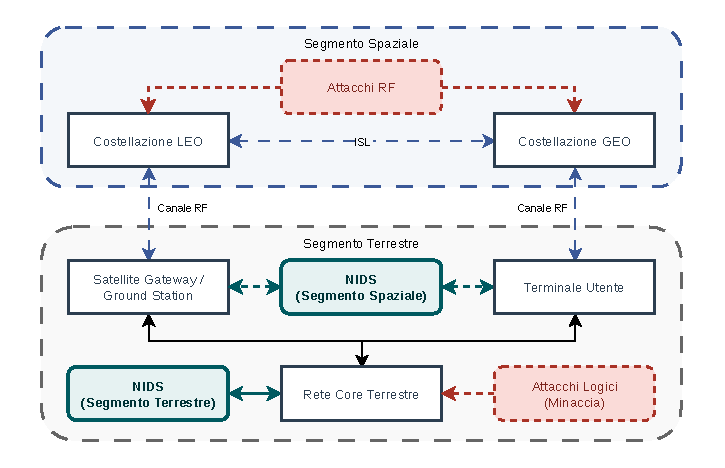
\includegraphics[width=\textwidth]{images/capitolo_2/sezione_1/architettura_ibrida.pdf}
    \caption{Architettura di rete integrata Terrestre-Spaziale: rappresentazione della superficie d'attacco e posizionamento dei punti di monitoraggio \textit{Network Intrusion Detection System} (NIDS).}
    \label{fig:architettura_ibrida}
\end{figure}

\section{Network Intrusion Detection Systems in Machine Learning}
\label{sec:ids_ml}

Muovendo da tali premesse, l'evoluzione delle minacce informatiche all'interno delle moderne infrastrutture di rete ha confermato l'inadeguatezza dei soli meccanismi di difesa perimetrali e di controllo degli accessi, determinando la necessità di adottare sistemi di rilevamento delle intrusioni basati su rete (\textit{Network Intrusion Detection Systems}, NIDS) per il monitoraggio continuo e profondo del traffico logico.
A differenza delle architetture Host-based (HIDS), progettate per analizzare i log locali e le chiamate di sistema del singolo elaboratore, un NIDS opera come un dispositivo hardware o un modulo software posizionato nei punti snodo dell'infrastruttura, con il compito di ispezionare passivamente o attivamente i flussi di dati in transito per identificare tentativi non autorizzati di accesso, violazioni delle politiche di sicurezza o compromissioni dell'integrità del canale \cite{hindy2020}.
Tradizionalmente, la rilevazione delle intrusioni nei NIDS si articola in due macro-approcci: l'ispezione basata sulle firme (\textit{Signature-based Detection}) e la rilevazione basata sulle anomalie (\textit{Anomaly-based Detection}).
Sebbene la prima garantisca un'elevata accuratezza nel riconoscere minacce note confrontando il traffico con un database di pattern malevoli prestabiliti, essa mostra un'intrinseca inefficacia di fronte ad attacchi inediti, noti come minacce \textit{Zero-Day}, e a varianti strutturali generate per eludere i controlli \cite{khraisat2019}, spostando l'interesse scientifico verso modelli analitici capaci di modellare il comportamento nominale del traffico di rete.

Proprio per superare la rigidità dei modelli deterministici basati su firme, l'integrazione delle tecniche di Machine Learning nei \textit{Network Intrusion Detection Systems} ha introdotto un paradigma adattivo e generalizzabile, in grado di analizzare la complessa e dinamica natura del traffico trasmissivo moderno.
Attraverso la formalizzazione di feature rilevanti — quali la frequenza dei pacchetti, la dimensione delle righe di intestazione e la distribuzione dei tempi di interarrivo —, un NIDS basato su Machine Learning costruisce una rappresentazione statistica del flusso informativo per rilevare deviazioni microscopiche riconducibili ad attività malevole senza la necessità di una firma preesistente \cite{hindy2020, khraisat2019}.
In questo contesto, la scelta metodologica orientata verso classificatori di tipo supervisionato rispetto a soluzioni non supervisionate garantisce vantaggi decisivi: laddove l'apprendimento non supervisionato risente di elevati tassi di falsi allarmi dovuti alla variabilità fisiologica della rete, i modelli supervisionati permettono di definire confini di decisione precisi e stabili, ottimizzando la discriminazione tra flussi leciti e malevoli sia in formulazioni biclasse sia in configurazioni multiclasse \cite{kilincer2021}.

\paragraph{NIDS in Machine Learning per le telecomunicazioni terrestri}
\label{prgf:ids_terrestri}

L'applicazione dei \textit{Network Intrusion Detection Systems} basati su Machine Learning al dominio delle telecomunicazioni terrestri risponde alla specifica esigenza di proteggere un'architettura ad altissima velocità e ad elevata densità di traffico.

% Nelle reti di terra, caratterizzate da canali in fibra ottica e ponti radio con larghezze di banda nell'ordine dei gigabit o terabit al secondo, i vettori d'attacco si manifestano frequentemente sotto forma di burst improvvisi di pacchetti, come negli attacchi \textit{Distributed Denial of Service} (DDoS), o di raffinate scansioni di porta distribuite (\textit{port scanning}) volte alla mappatura delle vulnerabilità \cite{hindy2020}.

I classificatori supervisionati all'interno dei NIDS si rivelano particolarmente efficaci in questo ambiente grazie alla loro capacità di sintetizzare le relazioni non lineari tra le \textit{feature} estratte a livello IP e di trasporto, mantenendo un'elevata efficienza computazionale in fase di inferenza e garantendo un contenuto tasso di falsi positivi \cite{kilincer2021}.
Tuttavia, l'analisi dello stato dell'arte in ambito terrestre evidenzia come gran parte della letteratura tenda a valutare tali modelli esclusivamente all'interno del medesimo dominio di addestramento, sottovalutando l'impatto del degrado prestazionale quando il sistema viene esposto a condizioni di canale differenti.

In quest'ottica, il primo contesto rilevante in letteratura è rappresentato dal lavoro di Tavallaee et al. \cite{tavallaee2009}, focalizzato sulla valutazione di modelli supervisionati per NIDS su dataset terrestri standardizzati.
Il punto di forza primario di questo contributo risiede nella rigida formalizzazione delle procedure di benchmarking e nella sistematica eliminazione dei bias di ridondanza del traffico, fornendo un riferimento metodologico fondamentale per la valutazione dei NIDS; tuttavia, il nostro approccio si differenzia nettamente in quanto lo studio di Tavallaee et al. confina la validazione a un ambiente rigorosamente intra-dominio, in cui addestramento e test condividono la medesima distribuzione di rete, senza analizzare il comportamento del classificatore di fronte a fenomeni di \textit{domain shift} né valutare l'impatto comparato tra la granularità di rilevamento binaria e multiclasse.
Un secondo contesto d'analisi essenziale è costituito dallo studio condotto da Sharafaldin et al. \cite{sharafaldin2018}, incentrato sull'impiego di classificatori supervisionati per NIDS su dataset terrestri moderni ad alta dimensionalità.
Il pregio fondamentale di tale ricerca consiste nel tracciamento dettagliato di vettori d'attacco complessi e multilivello all'interno di infrastrutture di rete eterogenee; ciononostante, il nostro lavoro prende le distanze da questa formulazione in quanto la validazione rimane eseguita esclusivamente all'interno del dominio terrestre di origine, omettendo di verificare la trasferibilità diretta del modello verso canali affetti da broad perturbazioni fisiche e trascurando la compensazione della scarsità di dati benevoli in domini di destinazione eterogenei.

\paragraph{NIDS in Machine Learning per le telecomunicazioni satellitari}
\label{prgf:ids_satellitari}

L'impiego dei \textit{Network Intrusion Detection Systems} basati su Machine Learning nelle comunicazioni satellitari deve affrontare vincoli operativi e dinamiche di canale profondamente differenti rispetto al contesto terrestre, derivanti dalle peculiarità fisiche e topologiche delle tratte orbitali.
Le reti spaziali sono penalizzate da elevati tempi di latenza di propagazione, larghezze di banda asimmetriche e da un'intrinseca suscettibilità al rumore atmosferico e ai fenomeni di \textit{fading} del segnale \cite{kodheli2021}.
In questo scenario, i tradizionali vettori d'attacco logici si sommano a minacce specifiche del canale ad etere, quali il \textit{jamming} mirato e l'iniezione non autorizzata di comandi \cite{nist2022}.
La scelta di adottare modelli supervisionati per i NIDS satellitari rispetto ad approcci non supervisionati si rivela fondamentale per evitare che le fluttuazioni stocastiche del canale radio spaziale vengano erroneamente classificate come anomalie malevole \cite{khraisat2019}; tuttavia, la vera criticità del dominio satellitare risiede nella marcata scarsità di dati etichettati relativi al traffico nominale (benevolo), che rende arduo l'addestramento di modelli nativi per lo spazio %\cite{siracusano2021}.

Nell'ambito della letteratura dedicata alla sicurezza dei collegamenti spaziali, un terzo contesto di riferimento di primaria importanza è rappresentato dal lavoro di Zhao et al. \cite{zhao2020}, incentrato sull'applicazione di classificatori supervisionati per il rilevamento di intrusioni e \textit{jamming} nei canali satellitari mediante NIDS dedicati.
Il pregio principale di questo contributo risiede nell'elevata accuratezza ottenuta nell'isolamento delle minacce a livello fisico ed etere in presenza di rumore elevato; tuttavia, il nostro approccio si diversifica in modo sostanziale poiché Zhao et al. assumono la disponibilità prioritaria di un dataset satellitare completo e perfettamente bilanciato per la fase di addestramento, ignorando la valutazione della trasferibilità di un modello addestrato su dati terrestri e la conseguente gestione dello scostamento distributivo.
Infine, un quarto contesto analitico rilevante è costituito dallo studio di Liu et al. \cite{liu2021}, che propone l'impiego di modelli supervisionati ad alta efficienza computazionale per NIDS destinati alla rilevazione di anomalie nei segmenti satellitari.
Il punto di forza di tale ricerca risiede nell'ottimizzazione dei tempi di esecuzione dell'inferenza, aspetto cruciale per il \textit{deployment} su nodi di bordo a risorse limitate; ciononostante, la nostra metodologia si differenzia poiché il lavoro di Liu et al. valuta il sistema esclusivamente in configurazione multiclasse all'interno di uno scenario stazionario, laddove il nostro studio analizza sia il livello di astrazione binario sia quello multiclasse, implementando strategie di iniezione mirata di dati per sopperire attivamente alla mancanza di un riferimento di traffico lecito nel dominio spaziale.

\begin{table}[H]
\centering
\small
\caption{Sintesi e confronto della letteratura principale sui NIDS basati su Machine Learning nei domini terrestre e satellitare.}
\label{tab:stato_arte_nids}
\begin{tabularx}{\textwidth}{l l l >{\RaggedRight\arraybackslash}X >{\RaggedRight\arraybackslash}X}
\toprule
\textbf{Riferimento} & \textbf{Dominio} & \textbf{Classificazione} & \textbf{Punto di Forza} & \textbf{Limite / Gap rispetto al nostro lavoro} \\
\midrule
Tavallaee et al. \cite{tavallaee2009} & Terrestre & Binaria / Multiclasse & Benchmarking rigido e pulizia bias (NSL-KDD) & Validazione ristretta all'ambito \textit{intra-domain}. \\
\addlinespace
Sharafaldin et al. \cite{sharafaldin2018} & Terrestre & Multiclasse & Traffico complesso e ad alta dimensionalità (CICIDS2017) & Assenza di analisi sulla trasferibilità del modello su canali perturbati. \\
\addlinespace
Zhao et al. \cite{zhao2020} & Satellitare & Binaria / Multiclasse & Isolamento di minacce a livello fisico (\textit{jamming}) & Assunzione di dataset satellitare bilanciato e ideale. \\
\addlinespace
Liu et al. \cite{liu2021} & Satellitare & Multiclasse & Efficienza computazionale per nodi di bordo & Valutazione solo multiclasse in scenario stazionario senza compensazione dati. \\
\bottomrule
\end{tabularx}
\end{table}

\vspace{0.5em}
\noindent
L'analisi dello stato dell'arte, i cui contributi principali e relativi limiti sono messi a confronto nella Tabella~\ref{tab:stato_arte_nids}, evidenzia come la progettazione di NIDS basati su Machine Learning per infrastrutture integrate necessiti di superare la visione stazionaria e omogenea prevalente in letteratura. 
Come illustrato nello schema concettuale di Figura~\ref{fig:domain_shift_concept}, l'estensione dei modelli dal dominio terrestre a quello satellitare richiede infatti di affrontare formalmente il degrado prestazionale causato dal cambio di distribuzione del traffico (\textit{domain shift}) e la strutturale scarsità di dati etichettati nello spazio, tematiche metodologiche che vengono analizzate nel dettaglio nella sezione seguente.

\begin{figure}[H]
    \centering
    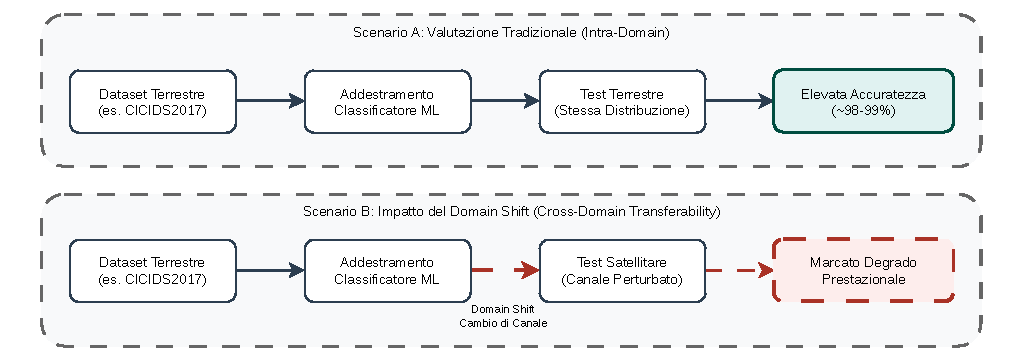
\includegraphics[width=\textwidth]{images/capitolo_2/sezione_2/domain_shift_concept.pdf}
    \caption{Confronto concettuale tra la valutazione tradizionale dei NIDS all'interno del medesimo dominio (\textit{intra-domain}) e l'effetto del \textit{domain shift} sulle prestazioni di classificazione nel passaggio al dominio satellitare (\textit{cross-domain}).}
    \label{fig:domain_shift_concept}
\end{figure}

\section{Adattamento di Dominio e Scarsità dei Dati}
\label{sec:domain_shift_data}

A completamento dell'analisi delle criticità connesse all'integrazione di sistemi di sicurezza basati sull'apprendimento automatico nei moderni ecosistemi di telecomunicazione, risulta indispensabile esaminare le problematiche metodologiche e teoriche legate alla variazione dei contesti operativi e alla disponibilità delle informazioni. 
La transizione da architetture trasmissive omogenee a scenari eterogenei impone infatti di superare i limiti strutturali associati non solo alla natura fisica dei canali, ma anche alla portabilità dei modelli analitici e alla disomogeneità statistica dei dataset di riferimento.

\paragraph{Il fenomeno del domain-shift nei sistemi NIDS}
\label{prgf:domain_shift_nids}

Dal punto di vista della teoria dell'apprendimento statistico, l'impiego di modelli di Machine Learning per la rilevazione delle intrusioni in contesti di rete eterogenei risente del fenomeno del disallineamento distributivo, noto in letteratura come \textit{domain shift} \cite{pan2009}. 
In termini formali, un dominio $\mathcal{D}$ è formalizzato come la coppia costituita da uno spazio delle \textit{feature} $\mathcal{X}$ e da una distribuzione di probabilità marginale $P(X)$, tale per cui $\mathcal{D} = \{\mathcal{X}, P(X)\}$. 
Assumendo uno spazio delle \textit{feature} condiviso ($\mathcal{X}_S = \mathcal{X}_T = \mathcal{X}$), dati un dominio di origine (\textit{source}) $\mathcal{D}_S = \{\mathcal{X}, P_S(X)\}$ e un dominio di destinazione (\textit{target}) $\mathcal{D}_T = \{\mathcal{X}, P_T(X)\}$, il fenomeno del \textit{domain shift} si verifica quando le distribuzioni marginali differiscono tra i contesti, ossia $P_S(X) \neq P_T(X)$ (\textit{covariate shift}), oppure quando muta la distribuzione condizionata delle classi $Y \in \mathcal{Y}$ rispetto alle osservazioni, ovvero $P_S(Y|X) \neq P_T(Y|X)$ (\textit{concept drift}) \cite{pan2009}. 
Nelle infrastrutture di telecomunicazione, tale discrepanza teorica si traduce nella variazione dei profili di traffico: la transizione dal canale terrestre a quello satellitare introduce ritardi di propagazione elevati, fluttuazioni della larghezza di banda e fenomeni stocastici di attenuazione atmosferica che alterano significativamente la distribuzione dei tempi di interarrivo e la struttura dei pacchetti %\cite{siracusano2021}. 
Tale scostamento sposta i vettori di test rispetto agli iperpiani di separazione appresi in fase di \textit{training}, provocando un grave degrado della capacità discriminativa del classificatore e un incremento incontrollato dei tassi di falso allarme \cite{farahani2021}. 
In letteratura, il problema dell'adattamento di dominio (\textit{domain adaptation}) viene affrontato principalmente mediante la ricerca di uno spazio latente comune o la minimizzazione di metriche di distanza statistica tra le distribuzioni \cite{wilson2020}. 
In quest'ambito, il lavoro di Wilson et al. \cite{wilson2020} fornisce un'analisi teorica esaustiva dei metodi di \textit{domain adaptation} volti a riallineare le distribuzioni marginali tra contesti differenti; il punto di forza di tale contributo risiede nella formalizzazione di modelli capaci di abbattere il \textit{bias} di dominio senza richiedere etichette nel contesto di destinazione, differenziandosi tuttavia dal nostro approccio in quanto la trattazione della letteratura è orientata prevalentemente ad ambienti omogenei e non affronta la specifica asimmetria strutturale e la marcata alterazione dei profili di traffico derivante dal trasferimento diretto tra il canale terrestre e quello orbitale.

\paragraph{Strategie di iniezione di dati per la mitigazione dello sbilanciamento}
\label{prgf:data_injection_nids}

Sul piano metodologico e teorico, l'adattamento di dominio deve confrontarsi con il problema dello sbilanciamento e della limitata disponibilità di informazioni etichettate nel dominio \textit{target}. 
Nelle applicazioni reali di Network Intrusion Detection, la scarsità di campioni appartenenti al dominio di destinazione costituisce un ostacolo primario all'addestramento di modelli nativi, configurando scenari di apprendimento semi-supervisionato o a pochi campioni (\textit{few-shot learning}) \cite{pan2009}. 
Nelle comunicazioni satellitari, tale criticità è esacerbata dalla profonda scarsità di tracce etichettate relative al traffico nominale del segmento spaziale, dovuta ai vincoli di riservatezza, all'elevato costo operativo e alla natura critica delle infrastrutture orbitali %\cite{siracusano2021}. 
Sebbene la letteratura proponga l'adozione di modelli puramente non supervisionati per ovviare alla mancanza di etichette, tali approcci teorici basati sulla sola stima della densità di probabilità mostrano un'intrinseca fragilità nei contesti ad alto rumore stocastico, scambiando le fisiologiche fluttuazioni del canale radio per attività malevole \cite{nist2022, khraisat2019}. 

Per preservare la capacità di definire confini di decisione rigidi tipica dei classificatori supervisionati, una strategia teoricamente solida consiste nell'adattamento del modello mediante l'iniezione mirata di dati del dominio \textit{target} nel dataset di origine (\textit{target data injection}) \cite{yang2021}. 
In termini formali, sia $\mathcal{D}_S = \{(x_i^S, y_i^S)\}_{i=1}^{N_S}$ il dataset di origine terrestre e $\mathcal{D}_T^{inj} = \{(x_j^T, y_j^T)\}_{j=1}^{N_T}$ la frazione ridotta di campioni satellitari iniettati ($N_T \ll N_S$), con $y_i^S, y_j^T \in \mathcal{Y}$. L'addestramento del modello $f(\cdot;\theta)$ viene condotto minimizzando una funzione di perdita (\textit{loss function}) congiunta $\mathcal{L}(\theta)$:
\begin{equation}
    \mathcal{L}(\theta) = \frac{1}{N_S} \sum_{i=1}^{N_S} \ell\left(f(x_i^S; \theta), y_i^S\right) + \alpha \frac{1}{N_T} \sum_{j=1}^{N_T} \ell\left(f(x_j^T; \theta), y_j^T\right)
    \label{eq:data_injection_loss}
\end{equation}
dove $\ell(\cdot)$ rappresenta la perdita istantanea (es. \textit{cross-entropy}) e $\alpha > 0$ è un iperparametro di ponderazione. L'ottimizzazione dell'Equazione~(\ref{eq:data_injection_loss}) permette di riallineare i confini di separazione e di inglobare la variabilità stocastica del canale di destinazione senza perdere la ricchezza informativa sugli attacchi complessi appresa dal dominio terrestre \cite{yang2021}. 
Tale approccio di iniezione mitiga lo sbilanciamento distributivo, garantendo un'elevata generalizzazione del classificatore sia nella discriminazione binaria sia nella caratterizzazione multiclasse delle minacce.

\section{Sintesi e Posizionamento del Lavoro}
\label{sec:sintesi_posizionamento}

L'analisi approfondita dello stato dell'arte e della letteratura di riferimento mette in luce una marcata frammentazione nella trattazione della sicurezza delle reti di telecomunicazione mediante strumenti di apprendimento automatico. 
Da un lato, la gran parte degli studi dedicati ai \textit{Network Intrusion Detection Systems} confina la validazione dei classificatori all'interno di ambienti stazionari e omogenei, assumendo implicitamente che i dati di addestramento e di test condividano la medesima distribuzione statistica e focalizzandosi in modo pressoché esclusivo sul dominio terrestre \cite{tavallaee2009, sharafaldin2018}. 
Dall'altro lato, i rari contributi orientati alla protezione delle comunicazioni spaziali presuppongono la disponibilità prioritaria di dataset satellitari completi, bilanciati e nativi, ignorando sia le marcate limitazioni operative connesse alla scarsità di tracciati di traffico nominale etichettato, sia l'impatto del disallineamento distributivo derivante dal trasferimento dei modelli tra canali trasmissivi eterogenei \cite{zhao2020, liu2021}. 
Inoltre, sebbene la letteratura teorica sull'adattamento di dominio fornisca quadri concettuali consolidati per la mitigazione del \textit{domain shift}, la sua applicazione pratica ai contesti di rete integrati rimane scarsamente esplorata, specialmente in relazione alla risposta comparata tra formulazioni di classificazione binaria e multiclasse \cite{pan2009, wilson2020}.

Alla luce di tali evidenze, il presente lavoro di tesi si posiziona nello spazio metodologico non ancora esaminato dalla letteratura, proponendo un'indagine sistematica sulla trasferibilità dei modelli di \textit{Machine Learning} supervisionati dal dominio terrestre a quello satellitare. 
L'elemento centrale dell'approccio proposto risiede nel superamento del vincolo di stazionarietà, valutando quantitativamente il degrado delle prestazioni generato dalle variazioni fisiche e temporali del canale radio (come schematizzato in Figura~\ref{fig:domain_shift_concept}) e analizzando contemporaneamente sia la capacità discriminativa di base (classificazione binaria) sia la caratterizzazione dettagliata delle minacce (classificazione multiclasse). 
Per fronteggiare la strutturale assenza di un riferimento di traffico nominale spaziale, la metodologia analizza l'efficacia di strategie di iniezione mirata e graduale di campioni del canale di destinazione all'interno del dataset primario terrestre, formalizzata attraverso la funzione di perdita congiunta dell'Equazione~(\ref{eq:data_injection_loss}). 
Tale soluzione dimostra come sia possibile riallineare gli iperpiani di separazione del classificatore e compensare la scarsità informativa del segmento satellitare, salvaguardando l'elevata capacità di discriminazione appresa sui complessi vettori d'attacco terrestri e fornendo un'architettura di monitoraggio adattiva e realmente operabile per le infrastrutture di telecomunicazione di nuova generazione \cite{yang2021}.